 \documentclass{beamer}

  \usepackage[utf8]{inputenc}
  \usepackage[T1]{fontenc}
  \usepackage{default}
  \usepackage{lmodern}
  \usepackage{color}
  \usepackage{listings}
  \usepackage{xcolor}
  \usepackage{caption}
  \usepackage{caption}
  \captionsetup[figure]{font=scriptsize, labelfont=scriptsize}
  
  \DeclareCaptionFont{white}{\color{white}}
\DeclareCaptionFormat{listing}{\colorbox{gray}{\parbox{\textwidth}{#1#2#3}}}
\captionsetup[lstlisting]{format=listing,labelfont=white,textfont=white}

\definecolor{vert}{rgb}{0.2,0.65,0}

  \usetheme{Copenhagen}
    \definecolor{vert}{rgb}{0.2,0.65,0}
    
    \setbeamertemplate{headline}
{%
  \leavevmode%
  \begin{beamercolorbox}[wd=.5\paperwidth,ht=2.5ex,dp=1.125ex]{section in head/foot}%
    \hbox to .5\paperwidth{\hfil\insertsectionhead\hfil}
  \end{beamercolorbox}%
  \begin{beamercolorbox}[wd=.5\paperwidth,ht=2.5ex,dp=1.125ex]{subsection in head/foot}%
    \hbox to .5\paperwidth{\hfil\insertsubsectionhead\hfil}
  \end{beamercolorbox}%
}

\setbeamertemplate{navigation symbols}{} 

  \title{Soutenance Projet de Master}
  \author{Romain Mencattini}
  \institute{Université de Genève}
  \date{\today}
  
    \AtBeginSection[]
  {
    \begin{frame}
    \frametitle{Sommaire}
    \tableofcontents[currentsection, hideothersubsections, pausesubsections]
    \end{frame} 
  }

\begin{document}

  %%%%%%%%%%%%%%%%%%%%%%
  %%% Page de Garde %%%%
  %%%%%%%%%%%%%%%%%%%%%%
  \begin{frame}
  \titlepage
  \end{frame}

	\section{Introduction} % => ~ 2 + 6
	
	\begin{frame}
		\frametitle{Notions de finance}
		Définition du FOREX\footnote{Source : \url{https://www.investopedia.com/terms/f/forex.asp}}: 
		\begin{quote}
			Forex (FX) is the market in which currencies are traded. The forex market is the largest, most liquid market in the world, with average traded values that can be trillions of dollars per day. It includes all of the currencies in the world.
		\end{quote}
	\end{frame}

	\begin{frame}
	\frametitle{Notions de finance}
	Propriétés du marché :
		\begin{itemize}
			\item Acteurs : les banques commerciales, les entreprises, les institutions financières non-bancaires et les ménages.
			\item Respecte la règle des trois unités.
			\item Outils possibles : \textit{spot}, \textit{futur} et \textit{option}.
	\end{itemize}
	\end{frame}

	\begin{frame}
		\frametitle{Notions de \textit{Machine learning}}
		Définition formelle du \textit{Machine learning}\footnote{Source : "\textit{Machine learning}" by Tom M. Mitchell}:
		\begin{quote}
			A computer program is said to learn from experience E with respect to some class of tasks T and performance measure P, if its performance at tasks in T, as measured by P, improves with experience E.
		\end{quote}
	\end{frame}

	\begin{frame}
		\frametitle{Notions de \textit{Machine learning}}
		Notions importantes :
		\begin{itemize}
			\item Données d'entraînement et de test.
			\item Apprentissage supervisé.
			\item Apprentissage non-supervisé.
		\end{itemize}
	\end{frame}


	\begin{frame}
		\frametitle{Motivations}
		Principales motivations :
		\begin{itemize}
			\item Peu de recherche sur le \textit{machine learning} appliqué au FOREX.
			\item Prendre en main et améliorer une technique existante.
		\end{itemize}
	\end{frame}
	
%%%%%%%%%%%%%%%%%%%%%%%%%%%%%%%%%%%%%%%%%%%%%%%%%%%%%%%%%%%%%%%%%%%%%%%%%%%%%
	\section{Algorithme et Implémentation}
	
	\begin{frame}
		\frametitle{Introduction}
		\begin{figure}
			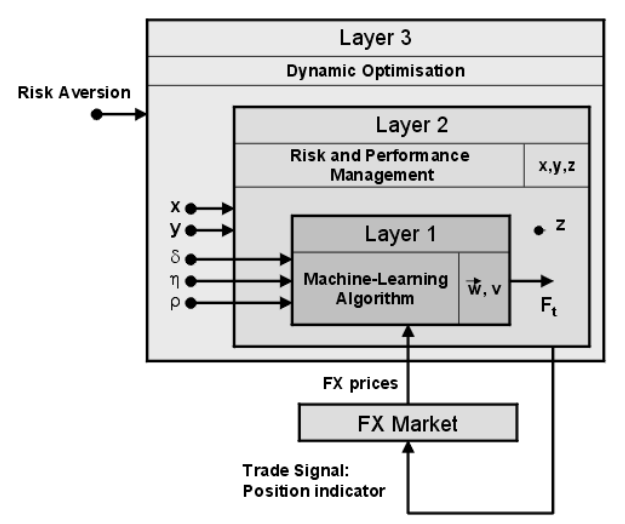
\includegraphics[scale=0.3]{../Rapport/images/exemple_nn_projet}
			\caption[]{Image provenant de l'article "\textit{An automated FX trading system using adaptive reinforcement learning}" de M.A.H. Dempster, V. Leemans }
		\end{figure}
	\end{frame}

	\begin{frame}
		\frametitle{Théorie \textit{Layer 1}}
		Éléments de la \textit{Layer 1}:
		\begin{itemize}
			\item Le calcul du signal : $$F_t = sign(\sum_{i=0}^{M} w_{i,t}r_{t-i} + w_{M + 1,t}F_{t-1} + v_t)$$
			\item L'optimisation s'effectue par descente du gradient. Le but est d'optimiser une estimation du \textit{Sharpe ratio} : $$\widehat{S}(t):= \frac{A_t}{B_t}$$ Où $A_t := A_{t-1} + \eta (R_t -A_{t-1})$ et $B_t := B_{t-1} + \eta (R_t^2 -B_{t-1})$
		\end{itemize}
	\end{frame}

	\begin{frame}
		\frametitle{Théorie \textit{Layer 2}}
		La \textit{Layer 2} est composée de:
		\begin{itemize}
			\item \textit{stop loss}.
			\item seuillage.
		\end{itemize}
		\begin{figure}
			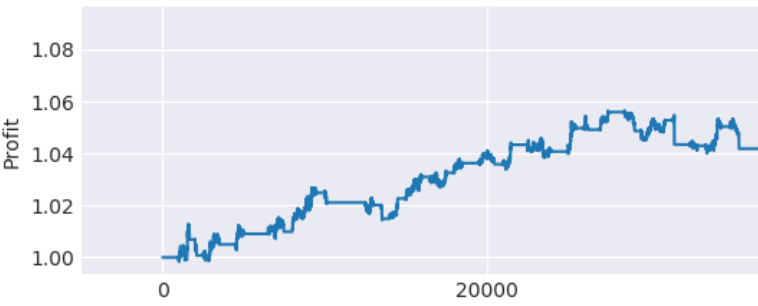
\includegraphics[scale=0.4]{../Rapport/images/stop_loss}
			\caption{Effet de la deuxième couche sur un profit cumulé de 3000 points.}
		\end{figure}
	\end{frame}

	\begin{frame}
		\frametitle{Théorie \textit{Layer 3}}
		Éléments de la \textit{Layer 3} :
		\begin{itemize}
			\item Les fonctions de coûts sont définies comme : $$\Sigma := \frac{\sum_{i=0}^N (R_i)^2 I(R_i < 0)}{\sum_{i=0}^N (R_i)^2 I(R_i > 0)}$$
			$$ U(\overline{R},\Sigma,\upsilon) := a\cdot(1-\upsilon)\cdot \overline{R} - \upsilon \cdot \Sigma$$ avec $\overline{R} := \frac{P_N}{N}$, $\upsilon$ l'aversion au risque et $a$ une constante.
			\item L'optimisation est donnée par : $$\max_{\delta, \eta, \rho, x, y} U(\overline{R};\Sigma: \delta, \eta, \rho, x, y; \upsilon)$$
			\item Afin de rendre le calcul possible, cette formule est préférée : $$\max\limits_{\delta} \max\limits_{\eta} \max\limits_{\rho} \max\limits_{x} \max\limits_{y} U(\bar{R};\Sigma : \delta, \eta, \rho, x, y; \nu)$$
		\end{itemize}
	\end{frame}

	\begin{frame}
		\frametitle{Implémentation}
		Différences avec la théorie :
		\begin{itemize}
			\item Fixer les valeurs initiales.
			\item Attribuer une valeur lorsqu'une fonction n'est pas définie.
			\item Compléter les manques.
		\end{itemize}
	\end{frame}

	\begin{frame}
		\frametitle{Problèmes}
		Les problèmes rencontrés sont :
		\begin{enumerate}
			\item Les poids ($w_i$) tendent vers l'infini.
			\item L'apprentissage est globalement inefficace.
			\item L'optimisation des méta-paramètres est bancale.
			\item Le programme ralenti au fil de l'exécution.
		\end{enumerate}
	\end{frame}

	\begin{frame}
	\frametitle{Solutions}
		Problème :
		\begin{quote}
			Les poids ($w_i$) tendent vers l'infini.
		\end{quote}
	
		Solution :
		\begin{quote}
			En changeant la descente du gradient par RMSProp : $$E[g^2]_t = 0.9 E[g^2]_{t-1} + 0.1 g^2_t$$ avec $$\theta_{t+1} = \theta_t + \frac{\rho}{\sqrt{E[g^2]_t + \epsilon}} g_t$$Cela permet d'éviter la divergence.
		\end{quote}
	\end{frame}

	\begin{frame}
		\frametitle{Solutions}
		Problème :
		\begin{quote}
			 L'apprentissage est globalement inefficace.
		\end{quote}
		
		Solution :
		\begin{quote}
			Par l'utilisation du \textit{Sharpe ratio} comme filtre, on diminue les périodes risquées et les pertes.
		\end{quote}
	\end{frame}

	\begin{frame}
		\frametitle{Solutions}
		Problème :
		\begin{quote}
			L'optimisation des méta-paramètres est bancale.
		\end{quote}
		
		Solution :
		\begin{quote}
			Fixer les valeurs initiales des méta-paramètres et effectuer une recherche aléatoire normale autour de ces dernières améliorent significativement l'optimisation.
		\end{quote}
	\end{frame}

	\begin{frame}
		\frametitle{Solutions}
		Problème :
		\begin{quote}
			Le programme ralenti au fil de l'exécution.
		\end{quote}
		
		Solution :
		\begin{quote}
			En évitant de stocker des éléments sur plusieurs itérations lorsque ce n'est pas nécessaire et en utilisant le parallélisme cela résous le problème.
		\end{quote}
	\end{frame}
	
%%%%%%%%%%%%%%%%%%%%%%%%%%%%%%%%%%%%%%%%%%%%%%%%%%%%%%%%%%%%%%%%%%%%%%%%%%%%%
	\section{Résultats}

	\begin{frame}
		\begin{figure}
			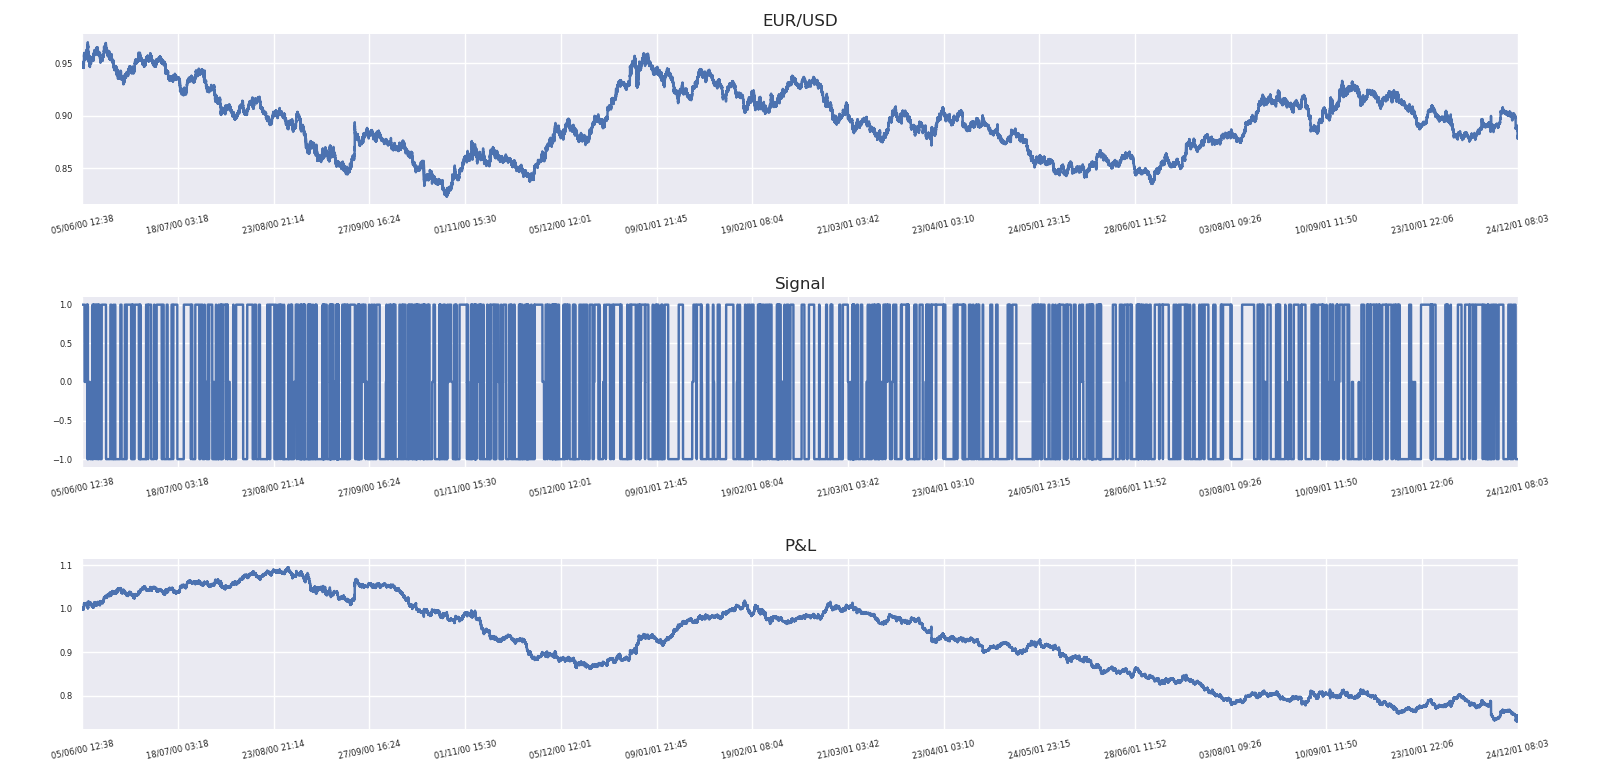
\includegraphics[scale=0.275]{../Rapport/res/eursud_2000-2001}
			\caption[Blup]{Cours EUR/USD entre le 01.06.2000 et le 31.09.2001, le signal d'achat prédit par l'algorithme ainsi que le \textit{p\&l} résultant de ces prédictions. Avec $|w| = 20$, $\delta = 0.001, \eta=0.001,\rho=0.01, x = 0.005, y=0.0001$.}
		\end{figure}
	\end{frame}

	\begin{frame}
		\begin{figure}
			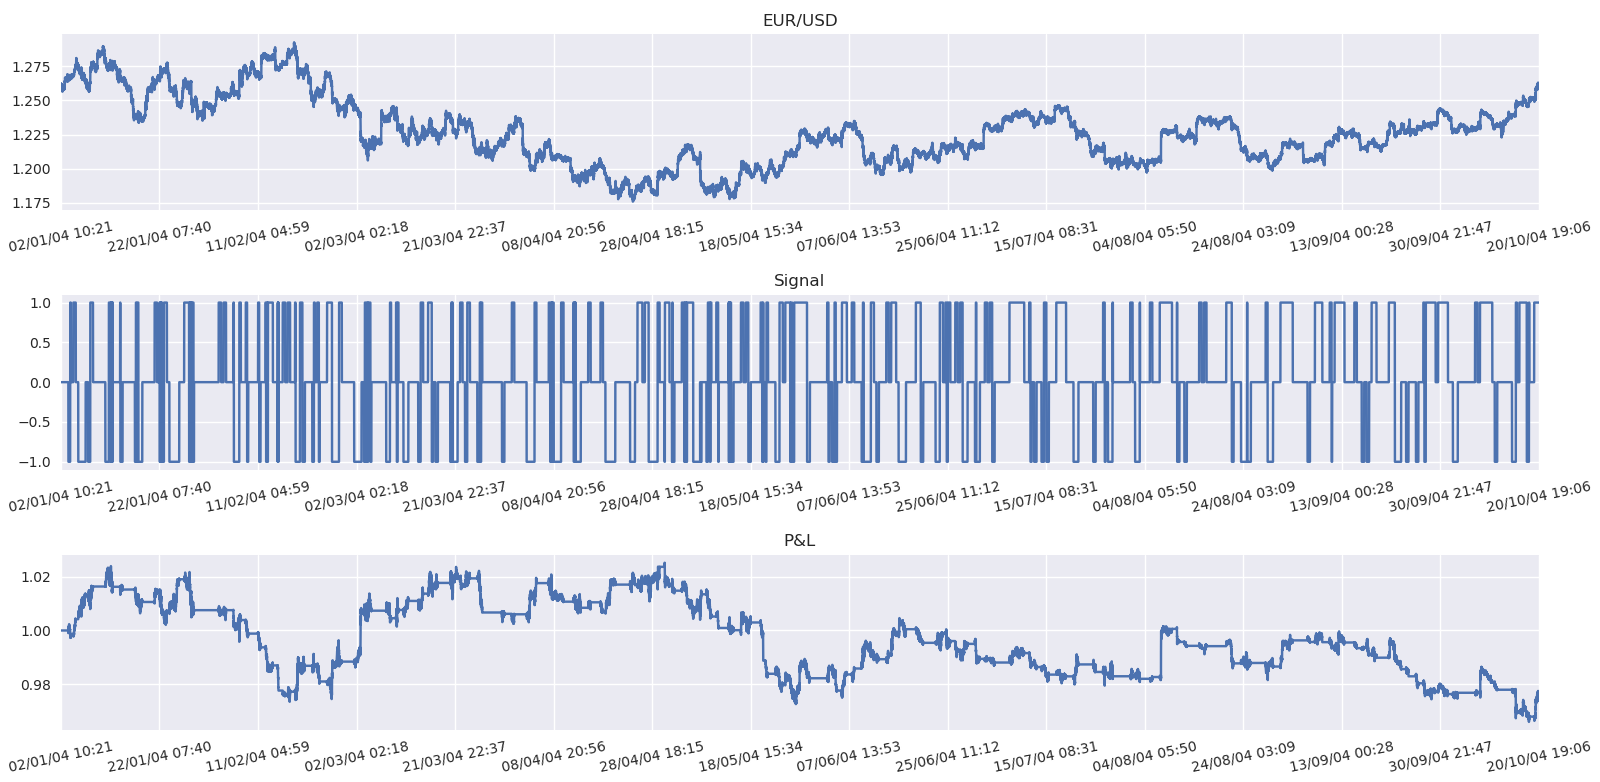
\includegraphics[scale=0.275]{../Rapport/res/eurusd_2004-2005}				\caption[Blup]{Cours EUR/USD entre le 01.01.2004 et le 31.10.2004, le signal d'achat prédit par l'algorithme ainsi que le \textit{p\&l} résultant de ces prédictions. Avec $|w| = 20$, $\delta = 0.001, \eta=0.001,\rho=0.01, x = 0.005, y=0.0001$.}
		\end{figure}
	\end{frame}

	\begin{frame}
		\begin{figure}
			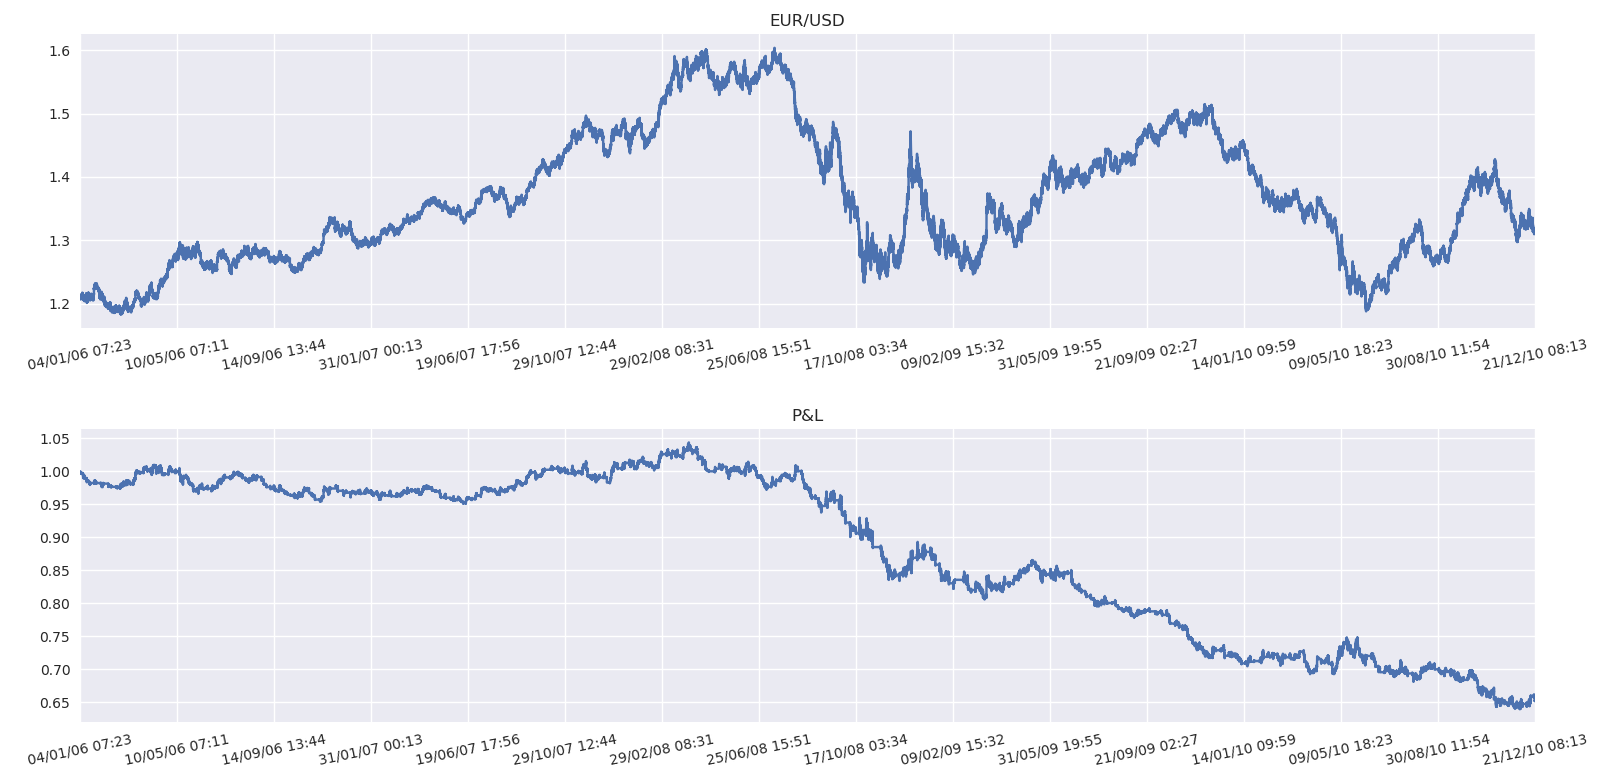
\includegraphics[scale=0.275]{../Rapport/res/eursud_2006-2010}
			\caption[Blup]{Cours EUR/USD de 2006 à 2010 et le \textit{p\&l} résultant des prédictions de l'algorithme. Avec $|w| = 20$, $\delta = 0.001, \eta=0.001,\rho=0.01, x = 0.005, y=0.0001$.}
		\end{figure}
	\end{frame}

	\begin{frame}
		\frametitle{Vitesse d'exécution}
		Temps d'exécution des différentes parties du programme :
		\begin{table}
			\centering
			\begin{tabular}{|l|c|}
				\hline
				 & Temps ($\mu s$)\\
				\hline
				Calcul $F_t$ & 25.5\\
				\hline
				Descente du gradient & 83\\
				\hline
				Optimisation des paramètres (après 200 itérations) & 220 \\
				\hline
				Optimisation des paramètres (après 2 itérations) & 2139 \\
				\hline
			\end{tabular}
		\caption{Temps d'exécution pour une étape de \textit{backtesting}, avec 2000 éléments d'entraînement et 500 de test, en moyenne sur 1000 runs.}
		\end{table}
	\end{frame}

%%%%%%%%%%%%%%%%%%%%%%%%%%%%%%%%%%%%%%%%%%%%%%%%%%%%%%%%%%%%%%%%%%%%%%%%%%%%%
	\section{Conclusion}
	
	\begin{frame}
		\frametitle{Pistes}
		Pistes envisageables :
		\begin{itemize}
			\item Ajouter des couches cachées au réseau de neurones.
			\item Améliorer l'optimisation des méta-paramètres.
			\item Implémenter une version alternative de la descente du gradient.
			\item Passer à des méthodes structurelles.
		\end{itemize}
	\end{frame}

	\begin{frame}
		\frametitle{Conclusion}
		En conclusion :
		\begin{itemize}
			\item Fonctionne localement mais pas globalement.
			\item Le projet est dans un état fonctionnel à partir d'un article incomplet.
			\item Cela fournit des pistes de recherches.
		\end{itemize}
	\end{frame}
	

\end{document}
